
%(BEGIN_QUESTION)
% Copyright 2011, Tony R. Kuphaldt, released under the Creative Commons Attribution License (v 1.0)
% This means you may do almost anything with this work of mine, so long as you give me proper credit

Determine how much voltage a DC voltmeter will register when connected between the specified test points in this 4-20 mA controller circuit for two different scenarios: one where everything is operating properly, and another where there is a {\it broken wire} between terminal TB1-3 and the positive input terminal of the controller.

$$\includegraphics[width=15.5cm]{i03419x01.eps}$$

Assume the pressure transmitter has been accurately calibrated to a range of 0 to 250 PSI, and is experiencing a steady process pressure of 184 PSI during the time you take your voltage measurements.  The controller is in manual mode, outputting a steady 73\% signal to the I/P transducer.

% No blank lines allowed between lines of an \halign structure!
% I use comments (%) instead, so that TeX doesn't choke.

$$\vbox{\offinterlineskip
\halign{\strut
\vrule \quad\hfil # \ \hfil & 
\vrule \quad\hfil # \ \hfil & 
\vrule \quad\hfil # \ \hfil \vrule \cr
\noalign{\hrule}
%
% First row
Test points & Voltage in healthy circuit & Voltage in faulted circuit \cr
%
\noalign{\hrule}
%
% Another row
TB1-9 to TB1-10 &  & \cr
%
\noalign{\hrule}
%
% Another row
TB1-6 to TB1-7 &  & \cr
%
\noalign{\hrule}
%
% Another row
TB1-2 to TB1-4 &  & \cr
%
\noalign{\hrule}
%
% Another row
Between transmitter terminals &  & \cr
%
\noalign{\hrule}
%
% Another row
TB1-9 to TB1-4 &  & \cr
%
\noalign{\hrule}
} % End of \halign 
}$$ % End of \vbox

\underbar{file i03419}
%(END_QUESTION)





%(BEGIN_ANSWER)

% No blank lines allowed between lines of an \halign structure!
% I use comments (%) instead, so that TeX doesn't choke.

$$\vbox{\offinterlineskip
\halign{\strut
\vrule \quad\hfil # \ \hfil & 
\vrule \quad\hfil # \ \hfil & 
\vrule \quad\hfil # \ \hfil \vrule \cr
\noalign{\hrule}
%
% First row
Test points & Voltage in healthy circuit & Voltage in faulted circuit \cr
%
\noalign{\hrule}
%
% Another row
TB1-9 to TB1-10 & {\bf 24 V} & {\bf 24 V} \cr
%
\noalign{\hrule}
%
% Another row
TB1-6 to TB1-7 & {\bf 2.666 V} & {\bf 2.666 V} \cr
%
\noalign{\hrule}
%
% Another row
TB1-2 to TB1-4 & {\bf 3.944 V} & {\bf 3.944 V} \cr
%
\noalign{\hrule}
%
% Another row
Between transmitter terminals & {\bf 20.06 V} & {\bf 20.06 V} \cr
%
\noalign{\hrule}
%
% Another row
TB1-9 to TB1-4 & {\bf 24 V} & {\bf 24 V} \cr
%
\noalign{\hrule}
} % End of \halign 
}$$ % End of \vbox

%(END_ANSWER)





%(BEGIN_NOTES)

{\bf This question is intended for exams only and not worksheets!}.

%(END_NOTES)


